

项目申请人主要从事伽辽金无网格法相关领域研究,并取得了一定的研究成果,已有国内外计算力学领域重要期刊发表论文20余篇,其中5篇发表于\textit{Computer Methods in Applied Mechanics and Engineering}。
相关系列工作不仅为本项目的研究奠定了坚实的研究基础,并积累了丰富的理论分析经验。具体的系列工作如下:

\subsubsection*{\bfseries (1)变分一致型伽辽金无网格法本质边界条件施加方案}
通常情况下,无网格近似形函数通常不具备插值性,无法直接施加本质边界条件,需通过基于弱形式的方案进行施加。
同时,变分一致型伽辽金无网格法也需要变分一致的本质边界条件施加方案配合,️以满足全域变分一致性。
针对该问题,申请人基于Hellinger--Reissner(HR)多变量变分原理发展了新型伽辽金无网格法本质边界条件施加方案。
该方法具有与传统Nitsche本质边界条件施加方法具有相类似的格式,同样具有一致项和稳定项。
图 \ref{fg:plate} 为所提方法在简支三角形方板问题中与传统罚函数法(Penalty)、Nitsche法的计算效率对比和人工参数敏感性分析。
相较于Nitsche法,所提方法一致项采用形函数的光滑导数替代传统无网格形函数高阶导数,在保证变分一致性的同时提高计算效率。
因此,在图 \subref*{fg:plate_time} 中所提HR方法在计算形函数及其导数上计算耗时大幅少于Nitsche,并于罚函数法相当。
而稳定项自然存在于所提方法弱形式中,无需额外引入稳定项,且稳定项中也不存在人工经验参数。
图 \subref*{fg:plate_alpha} 为计算精度和人工参数的关系,从图中可以看出,罚函数法和Nitsche法随人工参数取值不同,计算精度也随之改变。
取得最优精度时的人工参数在不同节点离散下也不相同,而所提HR型本质边界条件施加方案无需人工经验参数,即可达到传统方法的最优计算精度,使用过程简单方便。
此外,申请人还基于Hu--Washizu变分原理将该方法推广至薄壳问题中,发展薄壳结构准变分一致伽辽金无网格分析方法。

上述变分一致型伽辽金无网格法本质边界条件施加方案,为本项目研究时空混合离散伽辽金法时域末端虚位移本质边界条件施加方案奠定的重要的研究基础。

\begin{figure}[!h]
    \centering 
    \subfloat[计算效率对比]{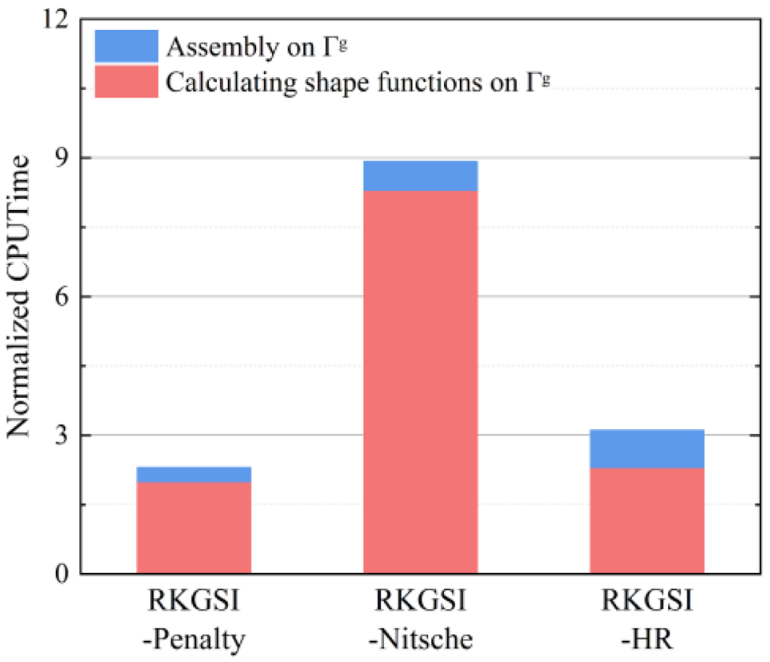
\includegraphics[width=0.444\textwidth]{figures/HRplate_time.png}\label{fg:plate_time}}
    \subfloat[人工参数$\alpha$敏感性分析]{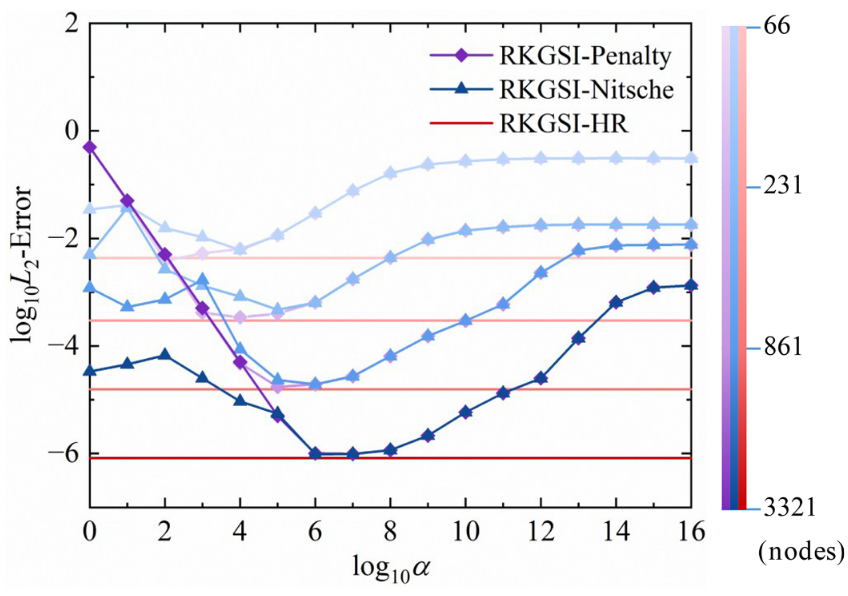
\includegraphics[width=0.546\textwidth]{figures/HRplate_alpha.png}\label{fg:plate_alpha}}
    \caption{HR变分一致型伽辽金无网格本质边界条件施加方案对比传统方案}
    \label{fg:plate}
\end{figure}

系列工作研究成果如下:

\vspace{-50pt}
\begin{thebibliography}{1}
	\providecommand{\bibauthor}[1]{#1}
	\providecommand{\bibeditor}[1]{#1}
	\providecommand{\bibtranslator}[1]{#1}
	\providecommand{\bibtitle}[1]{#1}
	\providecommand{\bibbooktitle}[1]{#1}
	\providecommand{\bibjournal}[1]{#1}
	\providecommand{\bibmark}[1]{#1}
	\providecommand{\bibcountry}[1]{#1}
	\providecommand{\bibpatentid}[1]{#1}
	\providecommand{\bibedition}[1]{#1}
	\providecommand{\biborganization}[1]{#1}
	\providecommand{\bibaddress}[1]{#1}
	\providecommand{\bibpublisher}[1]{#1}
	\providecommand{\bibinstitution}[1]{#1}
	\providecommand{\bibschool}[1]{#1}
	\providecommand{\bibvolume}[1]{#1}
	\providecommand{\bibnumber}[1]{#1}
	\providecommand{\bibversion}[1]{#1}
	\providecommand{\bibpages}[1]{#1}
	\providecommand{\bibmodifydate}[1]{#1}
	\providecommand{\bibcitedate}[1]{#1}
	\providecommand{\bibyear}[1]{#1}
	\providecommand{\bibdate}[1]{#1}
	\providecommand{\biburl}[1]{\newline\url{#1}}

	\bibitem[Wu et~al.(2024)Wu, Xu, Xu, and Basha]{wu2024}
	\textul{\textbf{Wu J}}, Xu Y, Xu B, Basha S~H.
	\newblock Quasi-consistent efficient meshfree thin shell formulation with
	  naturally stabilized enforced essential boundary conditions.
	\newblock \emph{Engineering Analysis with Boundary Elements}, 2024, 163:
	  641-655.

	\bibitem[Wu et~al.(2023)Wu, Wu, Zhao, and Wang]{wu2023}
	\textul{\textbf{Wu J}}, Wu X, Zhao Y, Wang D.
	\newblock A rotation-free {{Hellinger-Reissner}} meshfree thin plate
	  formulation naturally accommodating essential boundary conditions.
	\newblock \emph{Engineering Analysis with Boundary Elements}, 2023, 154:
	  122-140.

	\bibitem[吴俊超\ 等(2022)吴俊超, 吴新瑜, 赵珧冰, and
	  王东东]{Wu2022b}
	\textul{\textbf{吴俊超}}, 吴新瑜, 赵珧冰, 王东东.
	\newblock
	  {基于赫林格-赖斯纳变分原理的一致高效无网格本质边界条件施加方法}.
	\newblock 力学学报, 2022, 54: 3283-3296.

\end{thebibliography}

\subsubsection*{\bfseries (2)伽辽金无网格法精度分析}
由于无网格形函数的有理特性,伽辽金无网格法误差估计中将不可忽略由数值积分不准确引起的精度损失。
申请人采用泛函分析的手段,首次将变分一致性条件与伽辽金法正交性条件建立联系。
分析由数值积分满足变分一致性条件阶次和计算误差之间的关系,建立考虑数值积分误差的伽辽金无网格法误差估计。
该误差估计表达式分为两部分,一部分由形函数一致性条件确定,另一部分则由变分一致性条件控制。
该误差估计揭示了用于测试变分一致性条件的经典分片试验是如何影响计算误差。
图 \ref{fg:cube} 为三维方块势问题的伽辽金无网格法误差估计表达式的数值验证,算例中采用了满足变分一致性的再生核光滑梯度积分无网格法(RKGSI)和不满足变分一致性的高斯积分无网格法(GI)进行对比。
从分片试验图 \subref*{fg:cube_contour} 可以看出,仅有满足变分一致性的再生光滑梯度积分无网格法可通过分片试验,即使采用20点高斯积分(GI-20),传统方法依旧存在不可忽略误差。图 \subref*{fg:cube_slope} 为误差收敛率分析,该图可用所提伽辽金无网格法误差估计解释。当节点间距较大时,误差收敛率由一致性条件控制,高斯积分法可达到理论误差收敛率。当节点间距进一步加密,由一致性条件控制的误差迅速减小,高斯积分法误差收敛率转为由变分一致性条件控制而降低。再生光滑梯度理论框架可使两部分误差阶次保持一致,始终保持最优误差收敛效果。

\begin{figure}[!h]
    \centering 
    \subfloat[分片试验]{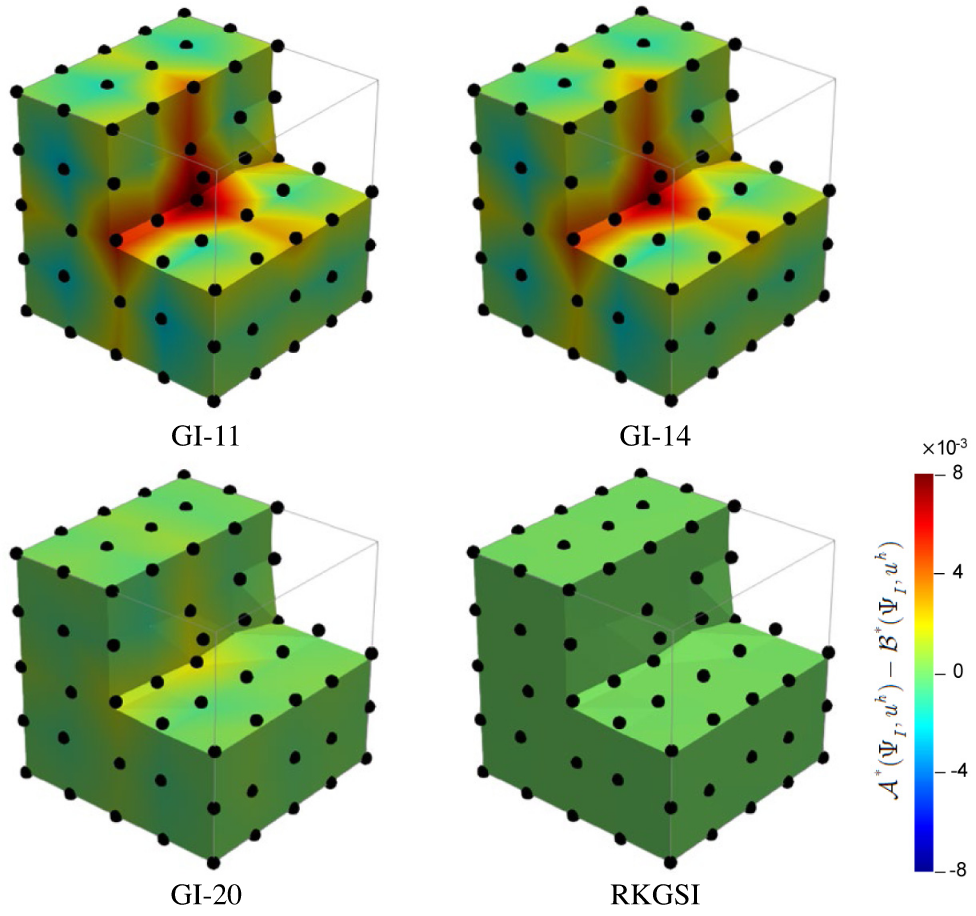
\includegraphics[width=0.45\textwidth]{figures/cube_contour.png}\label{fg:cube_contour}}
    \subfloat[误差收敛率分析]{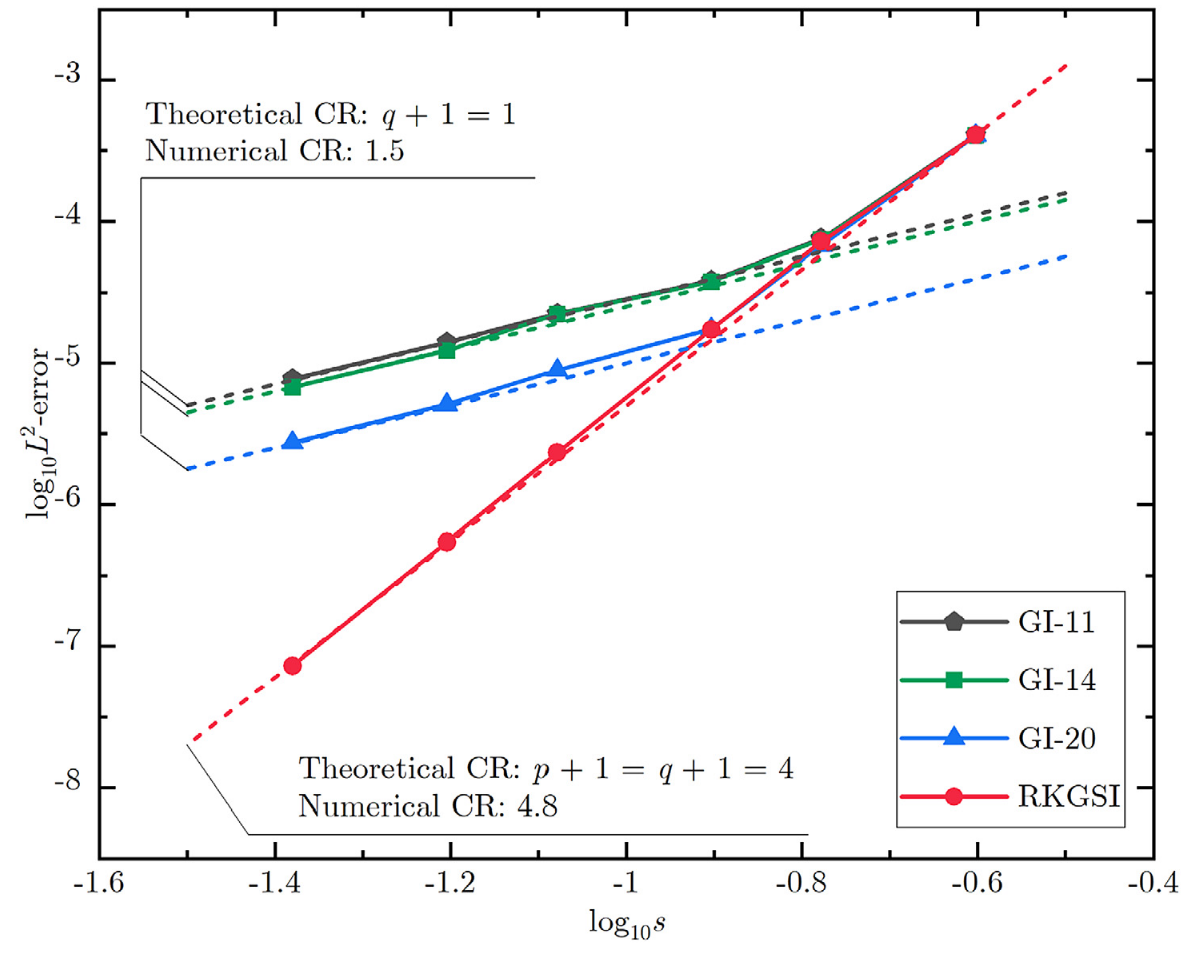
\includegraphics[width=0.55\textwidth]{figures/cube_slope.png}\label{fg:cube_slope}}
    \caption{伽辽金无网格法误差估计验证}
    \label{fg:cube}
\end{figure}

另一方面,申请人针对波动问题伽辽金无网格法振动分析,建立频率的局部截断误差估计表达式。
该误差估计表达式详细分析了如图 \subref*{fg:frequency_shape} 所示无网格形函数的周期性条件,并引入基于特征解的节点系数和形函数一致性条件进行化简。
基于此误差估计,将一致质量矩阵与局部质量矩阵进行优化组合,以消除低阶误差项,得到伽辽金无网格频率分析的高阶质量矩阵。
图 \subref*{fg:frequency_mass} 为高阶质量矩阵无网格法(HOM)与传统一致质量矩阵无网格法(CM)的频谱分析,结果表明高阶质量矩阵无网格法在波传播的任意方向上计算误差均优于一致质量矩阵伽辽金无网格法。

申请人在伽辽金无网格法误差估计中的研究结果,为本项目解决关键科学问题(2)如何确定时空混合无网格近似基向量阶次对求解稳定性的影响机理,提供了理论基础框架。
值得注意的是,频率局部截断误差估计中所采用的方案也是推导时空混合离散伽辽金无网格法局部截断误差估计中拟采用的研究方案。

\begin{figure}[!h]
    \centering 
    \subfloat[无网格形函数周期性]{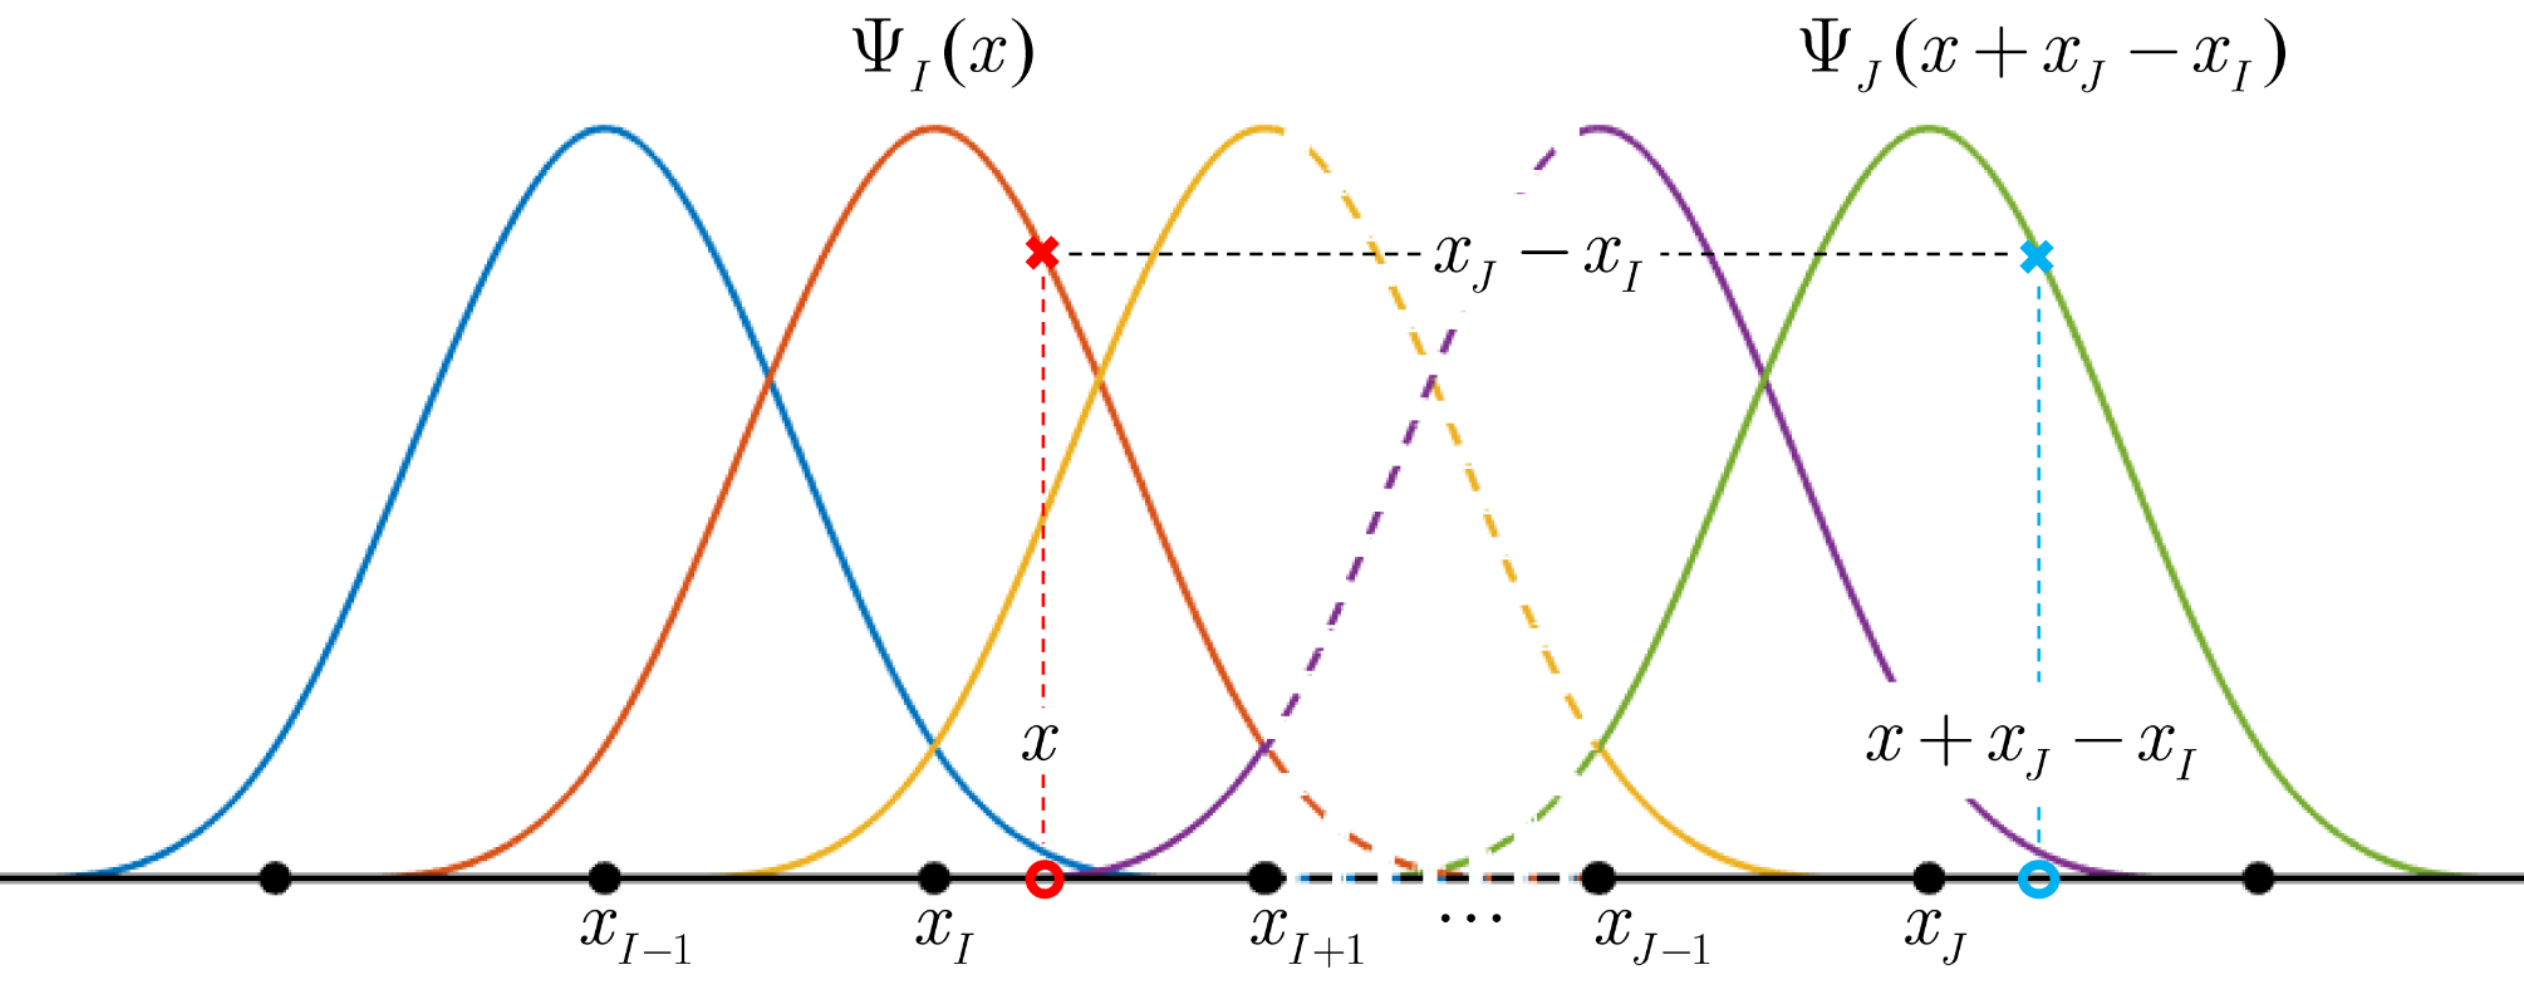
\includegraphics[width=0.7\textwidth]{figures/shape.png}\label{fg:frequency_shape}}
    \subfloat[无网格法频谱分析]{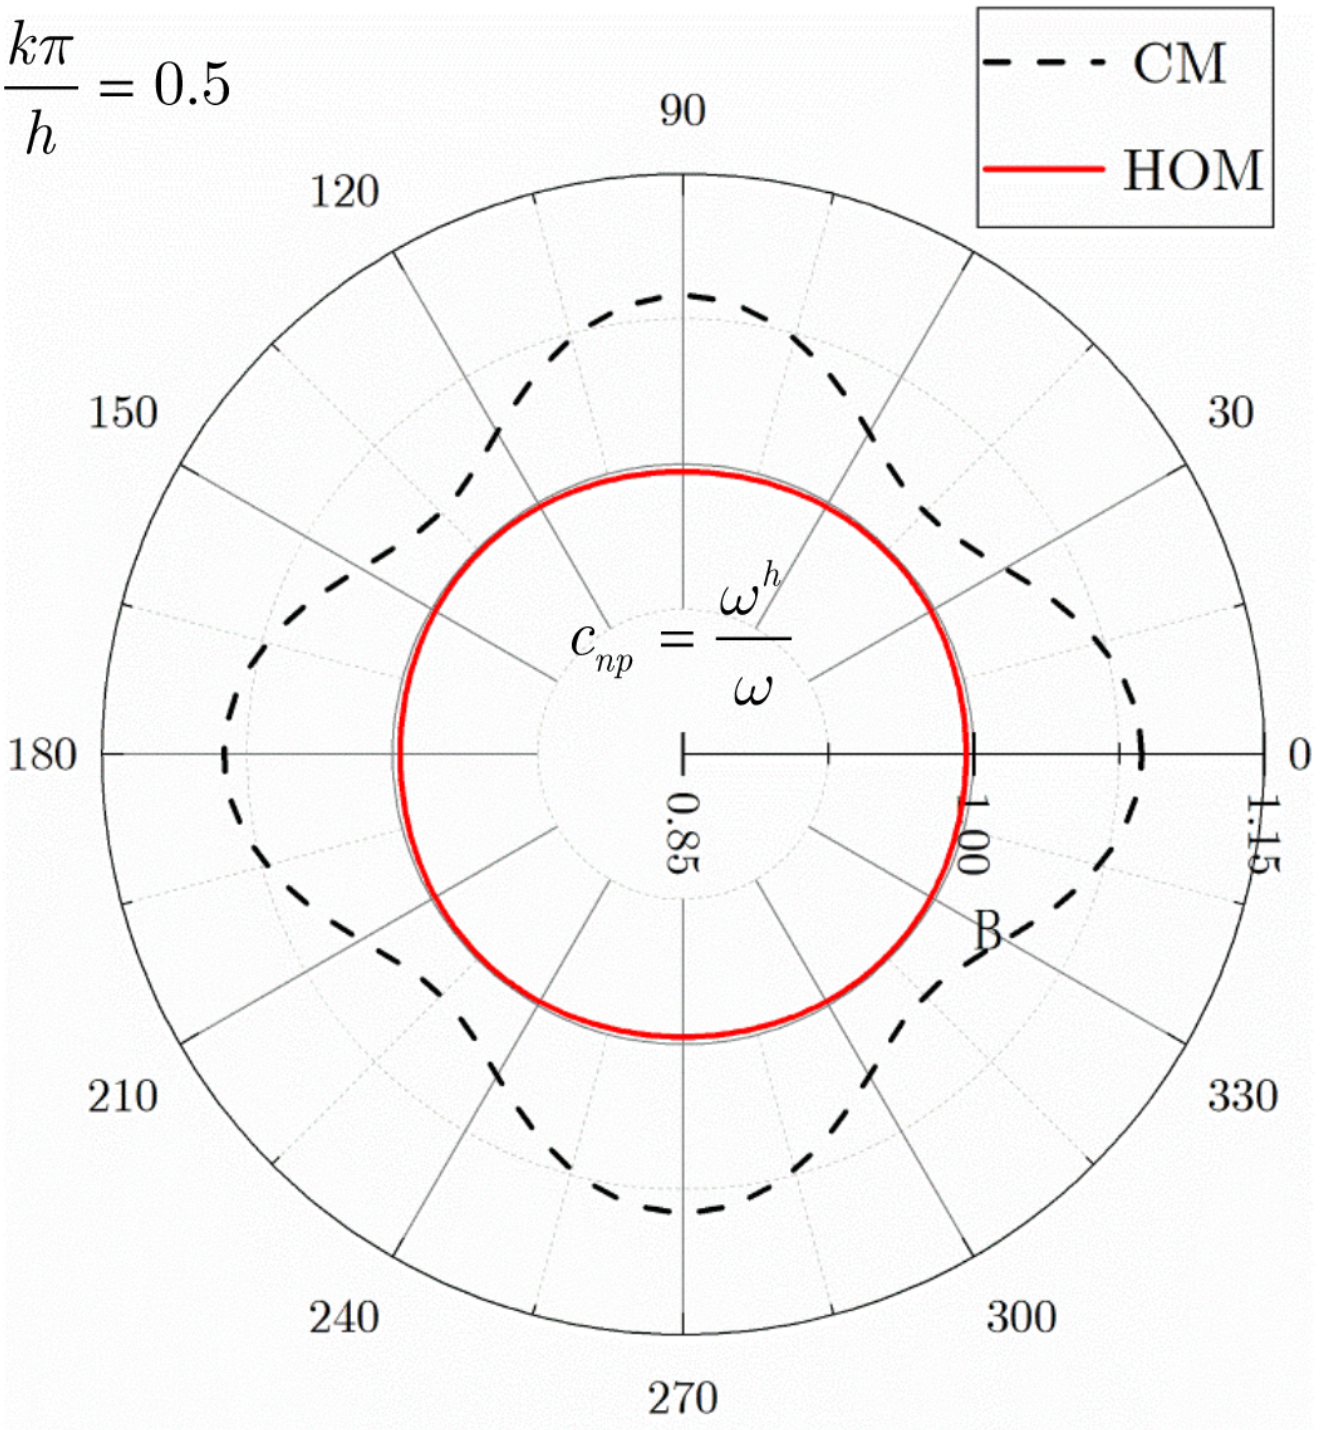
\includegraphics[width=0.3\textwidth]{figures/mass.png}\label{fg:frequency_mass}}
    \caption{伽辽金无网格法频率误差估计验证}
    \label{fg:frequency}
\end{figure}


系列工作研究成果如下:

\vspace{-50pt}
\begin{thebibliography}{1}
	\providecommand{\bibauthor}[1]{#1}
	\providecommand{\bibeditor}[1]{#1}
	\providecommand{\bibtranslator}[1]{#1}
	\providecommand{\bibtitle}[1]{#1}
	\providecommand{\bibbooktitle}[1]{#1}
	\providecommand{\bibjournal}[1]{#1}
	\providecommand{\bibmark}[1]{#1}
	\providecommand{\bibcountry}[1]{#1}
	\providecommand{\bibpatentid}[1]{#1}
	\providecommand{\bibedition}[1]{#1}
	\providecommand{\biborganization}[1]{#1}
	\providecommand{\bibaddress}[1]{#1}
	\providecommand{\bibpublisher}[1]{#1}
	\providecommand{\bibinstitution}[1]{#1}
	\providecommand{\bibschool}[1]{#1}
	\providecommand{\bibvolume}[1]{#1}
	\providecommand{\bibnumber}[1]{#1}
	\providecommand{\bibversion}[1]{#1}
	\providecommand{\bibpages}[1]{#1}
	\providecommand{\bibmodifydate}[1]{#1}
	\providecommand{\bibcitedate}[1]{#1}
	\providecommand{\bibyear}[1]{#1}
	\providecommand{\bibdate}[1]{#1}
	\providecommand{\biburl}[1]{\newline\url{#1}}

	\bibitem[Wu et~al.(2021)Wu and Wang]{wu2021}
	\textul{\textbf{Wu J}}, Wang D.
	\newblock An accuracy analysis of {{Galerkin}} meshfree methods accounting for
	  numerical integration.
	\newblock \emph{Computer Methods in Applied Mechanics and Engineering}, 2021,
	  375: 113631.

	\bibitem[Wu et~al.(2018)Wu, Wang, and Lin]{wu2018a}
	\textul{\textbf{Wu J}}, Wang D, Lin Z.
	\newblock A meshfree higher order mass matrix formulation for structural
	  vibration analysis.
	\newblock \emph{International Journal of Structural Stability and Dynamics},
	  2018, 18: 1850121.

\end{thebibliography}

\subsubsection*{\bfseries (3)变分一致型伽辽金无网格数值积分方案}
为解决伽辽金无网格法无法满足变分一致性引起精度下降问题,申请人发展了嵌套子域法和再生光滑梯度积分法。
尤其是再生光滑梯度积分法,该方法理论框架涵盖了所有以假定应变为基础的变分一致型数值积分方案。
在此框架下,采用与无网格基函数阶次配套的数值积分方案即可满足变分一致性。
同时,该框架还支持利用数值积分点在域积分和边界积分中的共享特性,对全域积分点数量进行优化,提高计算效率。
该方法经过近几年的发展,成功应用到了动力问题分析、Helmholtz方程分析、应变梯度结构分析、相场断裂模型分析等问题中。
本项目研究方案中拟将再生光滑梯度积分法推广应用至时空混合离散伽辽金无网格分析当中,以满足时空混合离散伽辽金弱形式的变分一致性,保证计算精度。
同时,将利用再生光滑梯度理论框架的优势,进一步优化四维时空区域数值积分点数量,提高整体分析的计算效率。

上述变分一致型伽辽金无网格数值积分方案的系列工作,为本项目研究时空混合离散伽辽金无网格法提供了扎实的理论基础。

系列工作研究成果如下:

\vspace{-50pt}
\begin{thebibliography}{1}
	\providecommand{\bibauthor}[1]{#1}
	\providecommand{\bibeditor}[1]{#1}
	\providecommand{\bibtranslator}[1]{#1}
	\providecommand{\bibtitle}[1]{#1}
	\providecommand{\bibbooktitle}[1]{#1}
	\providecommand{\bibjournal}[1]{#1}
	\providecommand{\bibmark}[1]{#1}
	\providecommand{\bibcountry}[1]{#1}
	\providecommand{\bibpatentid}[1]{#1}
	\providecommand{\bibedition}[1]{#1}
	\providecommand{\biborganization}[1]{#1}
	\providecommand{\bibaddress}[1]{#1}
	\providecommand{\bibpublisher}[1]{#1}
	\providecommand{\bibinstitution}[1]{#1}
	\providecommand{\bibschool}[1]{#1}
	\providecommand{\bibvolume}[1]{#1}
	\providecommand{\bibnumber}[1]{#1}
	\providecommand{\bibversion}[1]{#1}
	\providecommand{\bibpages}[1]{#1}
	\providecommand{\bibmodifydate}[1]{#1}
	\providecommand{\bibcitedate}[1]{#1}
	\providecommand{\bibyear}[1]{#1}
	\providecommand{\bibdate}[1]{#1}
	\providecommand{\biburl}[1]{\newline\url{#1}}

	\bibitem[Wang et~al.(2019)Wang and Wu]{wang2019a}
	Wang D, \textul{\textbf{Wu J}}.
	\newblock An inherently consistent reproducing kernel gradient smoothing
	  framework toward efficient {{Galerkin}} meshfree formulation with explicit
	  quadrature.
	\newblock \emph{Computer Methods in Applied Mechanics and Engineering}, 2019,
	  349: 628-672.

	\bibitem[Wang et~al.(2016)Wang and Wu]{wang2016b}
	Wang D, \textul{\textbf{Wu J}}.
	\newblock An efficient nesting sub-domain gradient smoothing integration
	  algorithm with quadratic exactness for {{Galerkin}} meshfree methods.
	\newblock \emph{Computer Methods in Applied Mechanics and Engineering}, 2016,
	  298: 485-519.

	\bibitem[Wu et~al.(2020)Wu, Wang, Lin, and Qi]{wu2020a}
	\textul{\textbf{Wu J}}, Wang D, Lin Z, Qi D.
	\newblock An efficient gradient smoothing meshfree formulation for the
	  fourth-order phase field modeling of brittle fracture.
	\newblock \emph{Computational Particle Mechanics}, 2020, 7: 193-207.

	\bibitem[Wang et~al.(2020)Wang, Wu, and Wang]{wang2020b}
	Wang J, \textul{\textbf{Wu J}}, Wang D.
	\newblock A quasi-consistent integration method for efficient meshfree analysis
	  of {{Helmholtz}} problems with plane wave basis functions.
	\newblock \emph{Engineering Analysis with Boundary Elements}, 2020, 110: 42-55.

	\bibitem[吴俊超\ 等(2016)吴俊超, 邓俊俊, 王家睿, and
	  王东东]{Wu2016d}
	\textul{\textbf{吴俊超}}, 邓俊俊, 王家睿, 王东东.
	\newblock 伽辽金型无网格法的数值积分方法.
	\newblock 固体力学学报, 2016, 3: 208-233.

	\bibitem[Du et~al.(2022)Du, Wu, Wang, and Chen]{du2022}
	Du H, \textul{\textbf{Wu J}}, Wang D, Chen J.
	\newblock A unified reproducing kernel gradient smoothing {{Galerkin}} meshfree
	  approach to strain gradient elasticity.
	\newblock \emph{Computational Mechanics}, 2022, 70: 73-100.

	\bibitem[付赛赛\ 等(2022)付赛赛, 邓立克, 吴俊超, 王东东, and
	  张灿辉]{Fu2022}
	付赛赛, 邓立克, \textul{\textbf{吴俊超}}, 王东东, 张灿辉.
	\newblock 再生光滑梯度无网格法动力特性研究.
	\newblock 应用力学学报, 2022, 39: 1065-1075.

\end{thebibliography}

综上所述,项目申请人及其团队在伽辽金无网格法的系列工作为本项目的顺利开展提供了良好的研究基础。

